\chapter{Kravspesifikasjoner}



Dette kapittelet vil ta for seg kravene som blir satt for funksjonelle krav i tillegg til supplementære krav. Disse skal hjelpe med å forstå hva programvarens grunnleggende oppgaver og hva som kan legges til.

	Funksjonelle krav \\ \\
	kommer mer









\section{Use Case}
Denne delen vil vise funksjonalitet kravene til programvaren gjennom use case diagrammer. I det første diagrammet har vi en generell oversikt over funksjonalitetene til programvaren 


\begin{figure}[h]
    \centering
    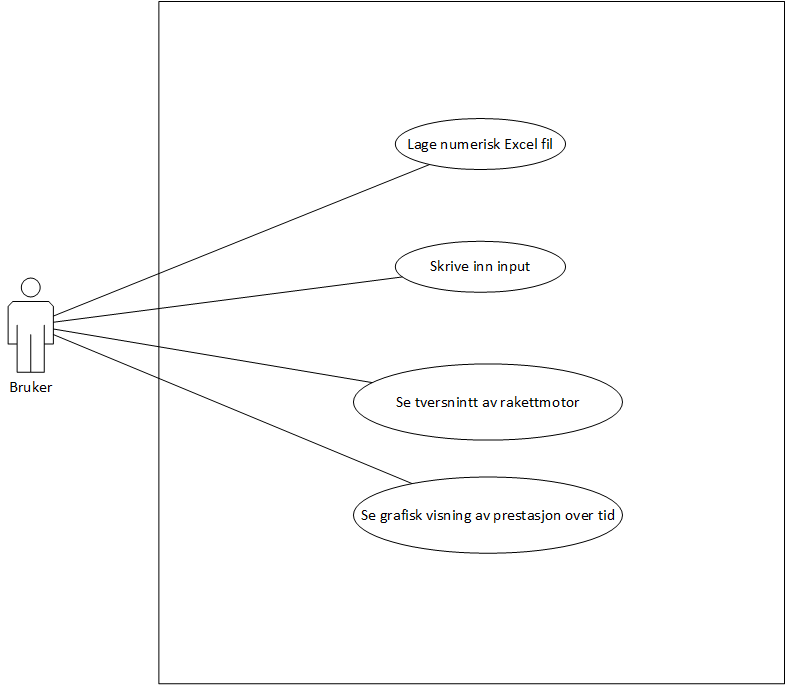
\includegraphics[width=\textwidth]{usecasepng}
    \caption{Use Case diagam}
    \label{fig:my_label}
\end{figure}

\section{Høynivå Use Case}
\begin{center}
  \begin{tabular}{ | l | p{8cm} | }
    \hline
    Use Case & Lage numerisk Excel fil \\ \hline
    Aktør & Bruker \\ \hline
    Hensikt & Lar brukeren eksportere data til en Excel fil\\ \hline
    Beskrivelse & Henter data om web, omkrets, portareal og webareal. Skaper Excel fil i filsystemt og legger hentet data inn i filen. \\
    \hline
  \end{tabular}
\end{center}

\begin{center}
  \begin{tabular}{ | l | p{8cm} | }
    \hline
    Use Case & Skrive inn input \\ \hline
    Aktør & Bruker \\ \hline
    Hensikt & Lar brukeren spesifisere parameter for modelleringen og beregningene\\ \hline
    Beskrivelse & Henter data fra brukeren og generer datamodeller og data basert på dette. \\
    \hline
  \end{tabular}
\end{center}

\begin{center}
  \begin{tabular}{ | l | p{8cm} | }
    \hline
    Use Case & Se tversnitt av rakettmotor \\ \hline
    Aktør & Bruker \\ \hline
    Hensikt & Viser datamodeller på skjermen\\ \hline
    Beskrivelse & Henter en ferdiggenerert datamodell som speiles og roteres før den vises. \\
    \hline
  \end{tabular}
\end{center}

\begin{center}
  \begin{tabular}{ | l | p{8cm} | }
    \hline
    Use Case & Se grafisk presentasjon over tid \\ \hline
    Aktør & Bruker \\ \hline
    Hensikt & Lar brukeren se hvordan brennoverflaten utvikler seg\\ \hline
    Beskrivelse & Viser en graf av omkrets over web (tid), basert på eksisterende beregninger. \\
    \hline
  \end{tabular}
\end{center}

\section{Design Krav}
Et av de meste etterspurte funksjonalitetene var en grafisk visning av hvordan rakettmotoren vil bli seendes ut. Denne visningen gir brukeren muligheten til å se hvor den initiale utskjæringen er, og hvor bred motoren er ved en visning av tankveggen. Mellom disse to blir brukeren vist hvordan den initiale utskjæringen vil forandre seg steg for steg. Avstanden mellom hvert steg har blitt definert av brukeren, sammen med den initiale utskjæringen. 


\subsection{2D Modell} 
Brukeren skal kunne bygge opp en komplett drivstofftank, med komplett brennstoffprofil, basert på forhåndsdefinerte segmenter med gitte parametere for modifisering. \\ \\
Segmentene med parametere er:
\begin{itemize}
    \item Ytre og indre radius på sylinderform
        \begin{itemize}
            \item Den ytre radiusen er der brennstoffet møter innsiden av tanken.
            \item Den indre radiusen er hvor brennstoffet møter brennkammeret.
        \end{itemize}
    \item Utformingen av stjerneform
        \begin{itemize}
            \item Hver arm er parallell og enden er avrundet.
            \item Brukeren kan endre på bredden og lengden på hver arm og antall armer.
            \item Vinkelen mellom hver arm er lik, så antallet armer og størrelsen på hver vil implisitt bestemme vinkelen.
        \end{itemize}
\end{itemize}



	



\subsection{Beregning}
En av de viktigste delene av programvaren er beregningen av forbrenningen i tanken, hvis denne er unøyaktig er programvaren nær verdiløs. Vi skal utvikle en algoritme for hvert segment brukeren kan legge inn i tanken.	\clearpage
\subsection{Presentasjon}
\begin{itemize}
    \item Numerisk output\\
    
    Nammo vil ha muligheten til å få resultatene levert i et numerisk Excel format, der de får effekten over tid presentert i en tabell. Dette skal kunne brukes som input til andre programmer, så det nøyaktige formatet må bestemmes etter nærmere samtaler med Nammo.\\
    \item Graf\\
    
    Når brukeren har laget sin versjon av brennstoffet skal resultatene vises i en graf umiddelbart. Grafen vil kun vises så lenge modellen er komplett, før dette og om brukeren fjerner et segment vil grafen ikke vises. Så lenge modellen er komplett skal alle endringer oppdatere grafen med en gang.
    
\end{itemize}

	\subsection{Valg av plattform}
Vi ønsket at programvaren skulle ha så få begrensninger som mulig, men programvaren er kun tilgjengelig på Windows maskiner. Nammo hadde planer om å kjøre programvaren på deres arbeidsmaskiner som alle kjører nyeste versjon av Windows. Vi valgte derfor å ikke gjøre programvaren kompatibel med flere plattformer. Dette ble nedprioritert fordi Nammo ikke hadde behov for kryssplattform funksjonalitet og vi prioriterte den grunnleggende funksjonaliteten.


\subsection{Brukervennlighet}
Brukervennlighet er noe vi har satt stor fokus på, det var viktig for oss å skape et produkt som ga brukeren en glede under bruk. Hvis programvaren er tungvint å bruke vil den ikke blir brukt, vi setter derfor brukervennlighet på samme nivå som funksjonalitet. Det er derfor viktig for oss definere hva brukervennlighet betyr, ettersom ordet i seg selv er litt vagt. Jacob Nilsen definerer brukervennlighet i sin artikkel for Nilsen Norman Group[1]. I denne artikkelen forteller han at brukervennlighet er definert av fem komponenter(Learnability, Efficiency, Memorability, Errors, Satisfaction). Vi har valgt å ta for oss fire av disse her ( Learnability, Efficiency, Errors, Satisfaction ). Learnability definerer hvor lett det er for brukeren å plukke opp programvaren å bruke den. Efficiency definer hvor effektiv bruker kan bli etter bruker han har lært seg programvaren. Errors definerer hva som skjer når brukeren gjør feil. Klarer programvaren å håndtere inputen eller vil den krasje. i tillegg hvor vanskelig det er for brukeren å rette opp feilene som har blitt gjort. Satisfaction definerer hvordan brukeren trives under interaksjonen av programvaren, er den tung å bruke eller blir brukeren sittende med en godt følelse. \\ \\
For å lage vår programvare så brukervennlig som mulig har vi valgt å gi brukeren med en enkel og minimal framside. Brukeren blir møtt med en framside som tar i mot parametrene som definerer raketten. Brukeren trenger kun å oppgi disse å trykke kjør. Dette gjør at det ikke er noen mer kompliserte verktøy som kan øke effektiviteten for mer erfaren brukere. Når brukeren har oppgitt sine parametere blir fremsiden oppdatert og resultatet blir vist. Hvis brukeren har gjort noe feil vil han ikke bli straffet for det. Bruker har fortsatt muligheten til å endre parametrene som ble oppgitt. Denne effektive å enkle løsningen føler vi vil gi brukeren en god opplevelse under bruken.



\subsection{Språkstøtte}
Nammo er et internasjonalt firma som opererer i land som Norge, Sverige, Finland, Spania, Tyskland, India og USA. Nammo har kontorer i 12 forskjellige land over hele verden. Det er derfor viktig å utvikle et produkt som kan brukes av alle land. Nammo produserer mesteparten av sine rakettmotorer på sine lokaler i Raufoss, Norge og noen på sine lokaler i USA. Vi kan ut fra denne informasjonen anta at programvaren kommer til å bli brukt for det meste i Norge. Det er en liten sansynlighet for at den kan bli brukt i USA eller utenlandske arbeidere på Raufoss kan bruke programvaren. Programvaren bruker derfor engelsk i tillegg til at all kode og kommentering er skrevet på engelsk, hvis Nammo ønsket å videreutvikle programmet.

\subsection{Sikkerhet}
Programvaren vi har utviklet har ikke noen form for brukerkontroll. Nammo hadde ingen behov for noe sikkerhetstiltak eller identifikasjon av bruker ettersom det ikke er noe sensitiv informasjon i bruke under programmet og er mer et verktøy. Siden programvaren blir installert på en maskin og ikke blir brukt over internett er det liten fare for brudd av sikkerhet.

\subsection{Dokumentasjon og testing}
Nammo viste en interesse for å videreutvikle programvaren etter vår bacheloroppgave. Vi har derfor tatt hensyn til deres ønsker og satt opp en oversiktlig arkitektur som deler kildekoden opp i tre forskjellige grupper( Model, View, Controller ). MVC er en kjent og mye brukt i bransjen i dag. Vi har valgt å ta den i bruk for sin simplisitet i tillegg til sin popularitet. Vi mener at denne modeller gir kildenkoden en strukturert arkitektur som gir nye utviklere en god forståelse av funksjonaliteten.

	\subsection{Ytelse}
Nammo skal kjøre programvaren på sine vanlige arbeid laptoper, disse har en begrenset prosesseringskraft. Funksjonaliteten Nammo ønsker er krevende å er en av våre største utfordringer. Vi må ta hensyn til disse maskinene og effektivisere den grunnleggende algoritmen så den er så lett at den kan kjøre på brukerens maskin uten å skape frustrasjoner og påvirke brukervennlighet.

\subsection{Lisenser}
\begin{description}

\item \textbf{Python}\\
Utgitt av Python Software Foundation, under PYTHON SOFTWARE FOUNDATION LICENSE VERSION 2\cite{Python}
\item \textbf{TkInter}\\
Utgitt under Python lisensen, mens Tcl og Tk bibliotekene som TkInter laster inn er utgitt under BSD lisensen\cite{TkInter}
\item \textbf{Matplotlib}\\
Utgitt av Matplotlib Development Team under License agreement for matplotlib 2.0.2\cite{Matplotlib}
\item \textbf{Numpy}\\
Utgitt av NumPy developers under NumPy license\cite{Numpy}
\end{description}